\section{Introduction}
In this assignment, a serial implementation of the Conjugate Gradient Method (CGM) was provided, which required
parallelization. In order to parallelize this implementation OpenMPI and the MPI parallelization paradigm was used.

\section{Serial Analysis}
The serial implementation of the CGM was evaluated using the provided \lstinline[language=Julia]|lap2D_5pt_n1000.mtx| matrix. This matrix
was chosen as its large size allowed for obvious parallelization opportunities to be revealed. The \lstinline[language=Julia]|perf|
profiling tool was used to analyse the serial code's execution time. From the profiling results, the \lstinline[language=Julia]|mat_vec|
function was identified as the primary computational bottleneck, accounting for approximately 86.27\% of the total execution
time. Consequently, the serial fraction of the program was estimated to be 13.73\%. The testing for the serial and
parallel code were performed on the Jed Cluster with and Intel\(R\) Xeon\(R\) Platinum 8360Y CPU, running at  2.40 GHz.


These values along with Amdahl's and Gustafson's laws for strong and weak scaling were used to calculate a theoretical
upper bound on the possible speed-ups that could be achieved using parallelization. The speed-ups were calculated using
the following equations~\cite{AmdahlGustafson2023}: 
\begin{align*}
   \text{Amdahl's Law (Strong Scaling)} = \frac{1}{(1-\alpha) + \frac{\alpha}{p}} 
\end{align*}
Here $\alpha$ is the fraction of the code that can be parallelized and $p$ is the number of processors. Gustafson's
equations are as follows:
\begin{align*}
    \text{Gustafson's Law (Weak Scaling)} = (1-\alpha) + \alpha p 
\end{align*}

\begin{figure}[h!]
    \centering
    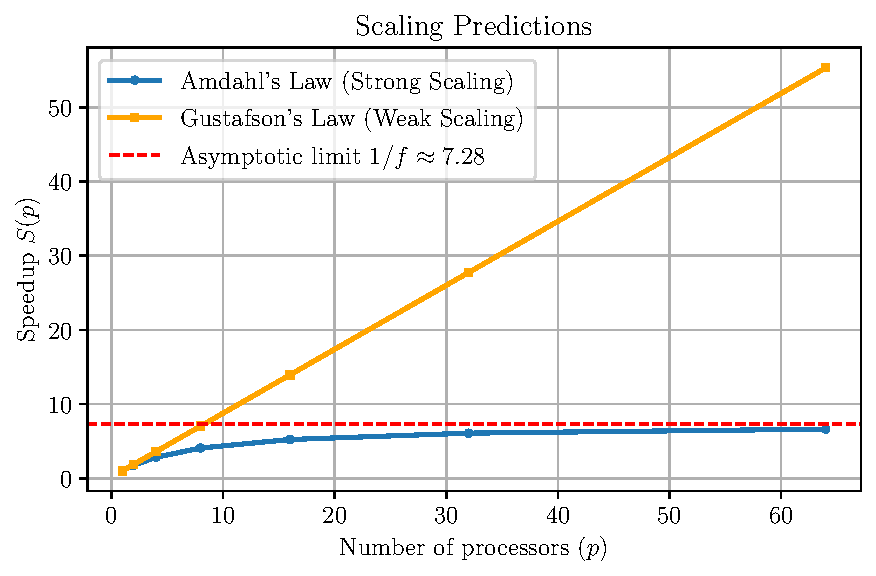
\includegraphics[width=\textwidth]{plots/scaling_laws.pdf}
    \caption{Strong and Weak Scaling Analysis using Amdahl's and Gustafson's Laws}
    \label{fig:AmdahlPlot}
\end{figure}
\FloatBarrier

\section{Parallel Modifications}
In order to parallelize the code with the least amount of communications, it was decided that the best course of action
would be to read in the matrix on processor 0 and then block distribute the row index, column index and value array to
each processor. Doing this when reading the matrix would implicitly parallelize the \lstinline[language=Julia]|mat_vec|
function and would reduce the communication needed to requiring just one \lstinline[language=Julia]|MPI_Allgather| after
each call to \lstinline[language=Julia]|mat_vec|, rather than a \lstinline[language=Julia]|MPI_Scatterv| and a
\lstinline[language=Julia]|MPI_Allgather| before and after the \lstinline[language=Julia]|mat_vec| calls. MPI message
packing and unpacking were also used to speed up this initial data transfer. This was enough to show some initial
improvements over the serial execution of the code, however, there was a lot more that could be done in the
\lstinline[language=Julia]|CGSolverSparse::solve()| function to further improve the parallelization of the code. Further
optimization was achieved through the use non-blocking transfers such as \lstinline[language=Julia]|MPI_Iallgatherv| as
well as combined communications such as \lstinline[language=Julia]|MPI_Reduce_scatter|. Using these combined
communications allows the MPI compiler to perform further optimizations when compiling the code. I also made use of
cblas operations such as \lstinline[language=Julia]|cblas_dcopy|, \lstinline[language=Julia]|cblas_daxpy| and
\lstinline[language=Julia]|cblas_ddot| to make use of the optimized implementations in the cblas library.

\section{Parallel Performance}
I had hoped all the changes that I had implemented would have significantly improved the runtime of the code over the
serial implementation. However, this was not the case. In my testing I noticed extremely poor scaling in the parallel
case. First I will showcase the performance graphs and then discuss the possible reasons and fixes for this. \\

For the strong scaling analysis I used the \lstinline[language=Julia]|lap2D_5pt_n1000.mtx| matrix and the
\lstinline[language=Julia]|lap2D_5pt_n200.mtx| matrix and then varied the processor count from 1 to 64. I decided to
stop at 64 since the timing results did not indicate any type of scaling. Most of the time, the parallel code took the
same time as the serial code and in some cases did slightly worse as can be seen in the graph below. \\

\begin{figure}[h!]
    \centering
    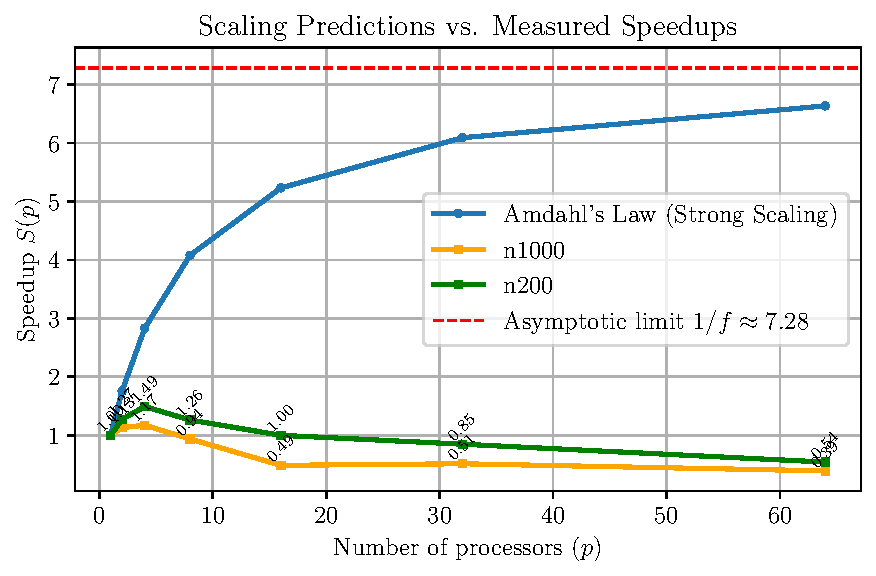
\includegraphics[width=\textwidth]{plots/strong_scaling.pdf}
    \caption{Strong Scaling Analysis}
    \label{fig:StrongScaling}
\end{figure}
\FloatBarrier
As can be seen from the graph above, minor performance gains can be achieved by switching from a serial code to a few
parallel processes. However, past 8 processors no further improvements are observed. \\ A similar story can also be seen
when performing a weak scaling analysis, as can be seen in the graph below. \\

\begin{figure}[h!]
    \centering
    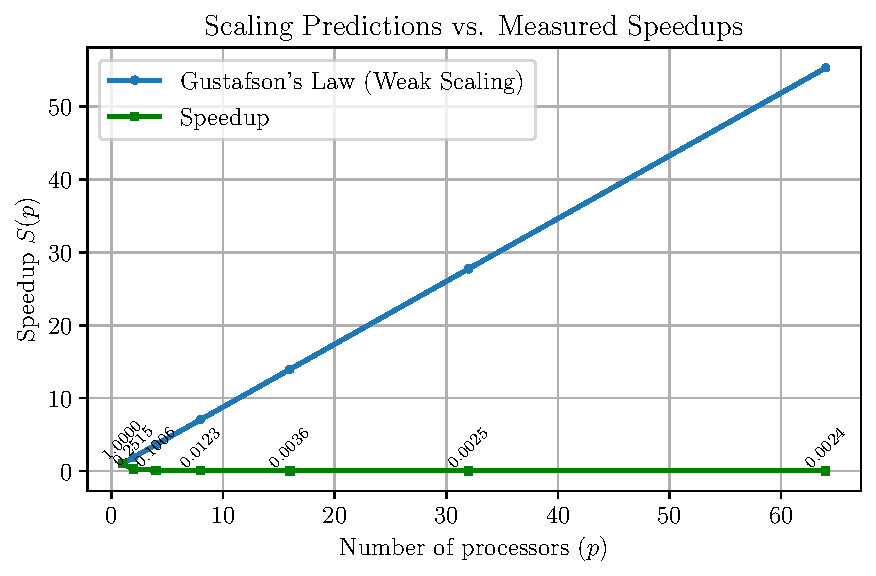
\includegraphics[width=\textwidth]{plots/weak_scaling.pdf}
    \caption{Weak Scaling Analysis}
    \label{fig:WeakScaling}
\end{figure}
\FloatBarrier

The raw results of the strong and weak scaling analysis can be seen in the tables below. \\

\begin{table}[h!]
    \centering
    \begin{tabular}{|c|c|c|c|c|c|c|c|}
        \hline
        \diagbox{Matrix Size}{\# Procs} & 1 & 2 & 4 & 8 & 16 & 32 & 64 \\ \hline
        n200 & 1.00 & 1.13 & 1.17 & 0.94 & 0.49 & 0.51 & 0.39 \\ \hline
        n1000 & 1.00 & 1.27 & 1.49 & 1.26 & 1.00 & 0.85 & 0.54 \\ \hline
    \end{tabular}
    \caption{Strong scaling speedup for different matrix sizes}
\end{table}

        
% weak scaling speed up data [1. 0.25147243 0.10058002 0.0122578  0.00355457 0.00252197 0.00238294]

\begin{table}[h!]
    \centering
    \begin{tabular}{|c|c|c|c|c|c|c|c|}
        \hline
        \# Procs & 1 & 2 & 4 & 8 & 16 & 32 & 64 \\ \hline
        speedup & 1. & 0.25147243 & 0.10058002 & 0.0122578 & 0.00355457 & 0.00252197 & 0.00238294 \\ \hline
    \end{tabular}
    \caption{Weak scaling speedup}
\end{table}

I suspect that the initial speedups come from the initial distribution of the matrix across all the processors. However,
this is quickly overshadowed by the large amount of collective communication required to calculate the intermediate
matrix vector products. In the \lstinline[language=Julia]|CGSolverSparse::solve| function there is a need to call
Allreduces on the dense vectors that are created from the sparse matrix vector products. For large linear systems this
cost is significant. Perhaps a better way to solve this issue would have been to create a sparse vector class and
impliment a sparse matrix vector product function. In this way we can still calculate a distributed matrix vector
product with all-to-all communication while avoiding the costs involved with communicating large vectors. I tried to
mitigate this mostly through the use of non-blocking communications, however the improvements from this were minor.
Another fix I had tried was re-ordering the calculations so that some work could be done in the time when a collective
communication was sent and when it actually needed to be received in order to be used in a calculation. Again the
improvements from this were minor.